\documentclass[10pt]{article} 
\usepackage[utf8]{inputenc}

%%% PAGE DIMENSIONS
\usepackage{geometry} 
\geometry{a4paper} 
\geometry{margin=.75in} 

%%% PACKAGES
\usepackage{booktabs} 
\usepackage{array} 
\usepackage{paralist}
\usepackage{verbatim} 
\usepackage{subfig} 
\usepackage{caption}
\usepackage{amsmath}
\usepackage{float}
\usepackage{color}
\usepackage[pdftex]{graphicx}

%%% HEADERS & FOOTERS
\usepackage{fancyhdr} 
\pagestyle{fancy} 
\renewcommand{\headrulewidth}{0pt} 
\lhead{}\chead{}\rhead{}
\lfoot{}\cfoot{\thepage}\rfoot{}

%%% ANIMATIONS
\usepackage{animate}

%%% SECTION TITLE APPEARANCE
\usepackage{sectsty}
\allsectionsfont{\sffamily\mdseries\upshape} 


%%% ToC (table of contents) APPEARANCE
\usepackage[nottoc,notlof,notlot]{tocbibind} 
\usepackage[titles,subfigure]{tocloft} 
\renewcommand{\cftsecfont}{\rmfamily\mdseries\upshape}
\renewcommand{\cftsecpagefont}{\rmfamily\mdseries\upshape} 

\title{Monte Carlo Methodology and the Wolff Algorithm: \newline The Ising Model Revisited}
\author{Mark Wittekind \& Drew Murray}

%\date{} % Remove the '%' before '\date{}' to display a given date or no date (if empty),
         % otherwise leave the '%' and the current date is printed 

\newcommand{\beq}{\begin{equation}} 
\newcommand{\eeq}{\end{equation}} 
\newcommand{\n}{\noindent} 


\begin{document}
\maketitle
\section{Introduction}

The Ising model consists of a collection of particles arranged in a lattice.  Each particle can have one of two spins, up or down, making a binary system.  The Wolff algorithm uses clustering to pseudo-randomly update the spins in a manner that resembles temperature demagnetization of physical binary systems.  By simulating the lattice's response to temperature for many different temperatures, many physical phenomena can be observed.


\section{Initial Conditions}

A periodic, 2D lattice of size 100x100 particles, evenly spaced and with identical spins, was initialized.  The simulation was then run for a range of pre-specified temperatures.  For each temperature, the lattice was reinitialized and the Wolff algorithm was subsequently run a large number of timesteps to ensure steady-state magnetization.

\beq
\label{eqn:equation1}
Timesteps = \frac{Tn}{2}
\eeq

where n is the number of particles in the system.

Although we do not know the explicit functional dependence of accuracy on temperature we do know the runtime depends exponentially on T.  Therefore a simple method to reduce runtime at lower temperatures while maintaining a reasonable degree of accuracy at higher temperatures is to vary the timesteps as a linear function of temperature.

\section{Runtime}

The Wolff algorithm creates clusters and flips the spin of all constituent particles.  It adds particles to the cluster semi-randomly dependent on temperature.

\subsection{Wolff Algorithm}

1) Choose a particle at random and flip its spin
2) Consider all nearest neighbors, add each neighbor with the same spin as the original particle to a queue with probability
\beq
\label{eqn:equation2}
P(T)=1-e^{\frac{-2J}{K_{b}T}}
\eeq
3) If the particle was added to the queue, flip its spin
4) Repeat from step 2 with the first particle in the queue as the 'chosen' particle

\subsection{Temperature Range}
We chose two temperature ranges to observe due to limitations on computation time:

\subsection{Magnetization versus Temperature}
We selected a relatively large range of temperatures (1-5) to explore when interested in the behavior of magnetization as a function of temperature.  Due to the larger range of temperatures we had to reduce the resolution in temperature steps to a delta T of .002 to hit a target runtime.

\subsection{Critical Temperature}
In looking for the critical temperature $T_c$ we could explore a smaller temperature range (2.2-2.4) with a higher resolution delta T of .00015.

\section{Results \& Analysis}
\subsection{Magnetization}
\subsubsection{Calculation}
Magnetization was normalized on the number of spin states in our lattice as follows:

\beq
\label{eqn:equation3}
m=|\frac{1}{n}\sum\limits_{i,j} s_{i,j}|
\eeq

\subsubsection{Behavior}
At temperatures far below $T_c$ we observe rapid oscillation of spin across the whole system.  This agrees with our expectations due to the lack of an external field establishing a distinction between spin up and down.


Near $T_c$ we observe a rapid drop in magnetization from 1 to zero.

At temperatures above $T_c$ we observe random spin states leading to an overall magnetization of approximately zero.  These observations are illustrated.

\begin{figure}[H]
\centering
\begin{minipage}{.75\textwidth}
\centering
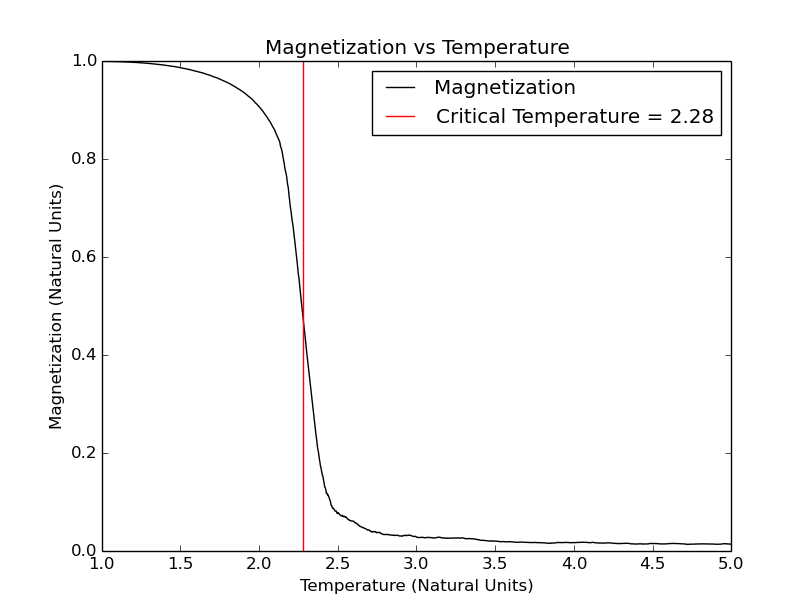
\includegraphics[width= \linewidth]{Mag_v_Temp.png}
\end{minipage}\hfill
\caption{Plot of magnetization versus temperature.}
\label{fig:figure1}
\end{figure}
\n
\subsection{Susceptibility}
Susceptibility is calculated as follows:

\beq
\label{eqn:equation4}
\chi=\frac{\partial \bar{m}}{\partial t}
\eeq

We utilized this calculation to find $T_c$ = 2.285 by locating the minimum of this plot.  This agrees with our expectations of a $T_c$ of around 2.2.

\begin{figure}[H]
\centering
\begin{minipage}{.75\textwidth}
\centering
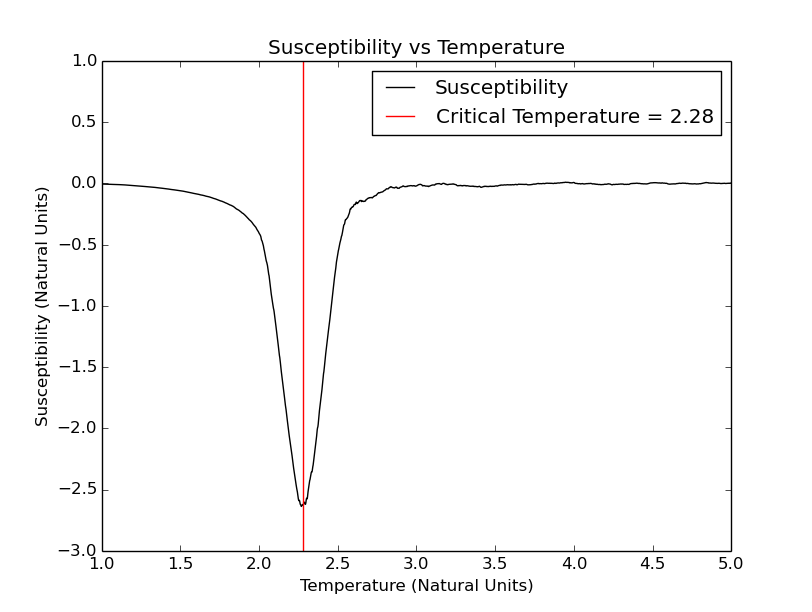
\includegraphics[width= \linewidth]{Sus_v_Temp.png}
\end{minipage}\hfill
\caption{Plot of susceptibility versus temperature.}
\label{fig:figure2}
\end{figure}
\n
\subsection{Internal Energy}
Internal energy is calculated as follows:

\beq
\label{eqn:equation5}
U=-J\sum\limits_{<i,j>} s_is_j
\eeq

This behaves similarly to m(T) as expected.

\begin{figure}[H]
\centering
\begin{minipage}{.75\textwidth}
\centering
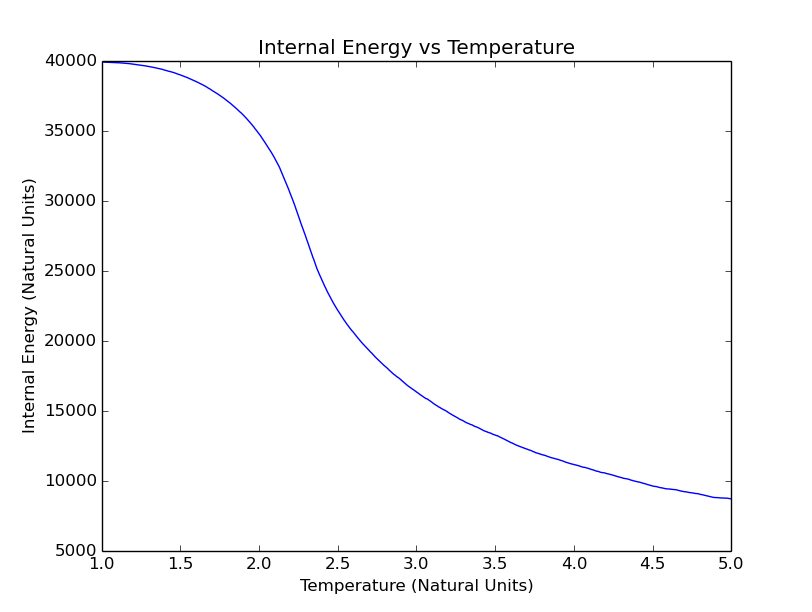
\includegraphics[width= \linewidth]{Internal_Energy_v_Temp.png}
\end{minipage}\hfill
\caption{Plot of internal energy versus temperature.}
\label{fig:figure3}
\end{figure}
\n
\subsection{Specific Heat}
Specific heat is calculated as follows:

\beq
\label{eqn:equation6}
\chi=\frac{\partial U}{\partial t}
\eeq

This behaves similar to $\chi(T)$ and centers on $T_c$.

\begin{figure}[H]
\centering
\begin{minipage}{.75\textwidth}
\centering
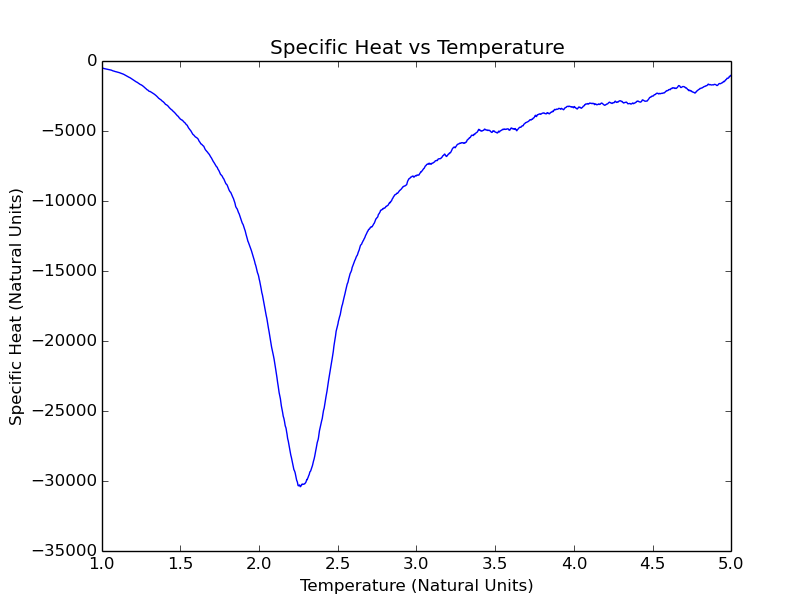
\includegraphics[width= \linewidth]{Specific_Heat_v_Temp.png}
\end{minipage}\hfill
\caption{Plot of specific heat versus temperature.}
\label{fig:figure4}
\end{figure}
\n
\n
\subsection{Critical Exponent}
The critical exponent $\gamma$ is defined as follows:


\beq
\label{eqn:equation7}
m\approx |T-T_c|^{\gamma}
\eeq

Using logarithms we can solve for $\gamma$:

\beq
\label{eqn:equation8}
\gamma \approx log(m-|T-T_c|)
\eeq

\begin{figure}[H]
\centering
\begin{minipage}{.75\textwidth}
\centering
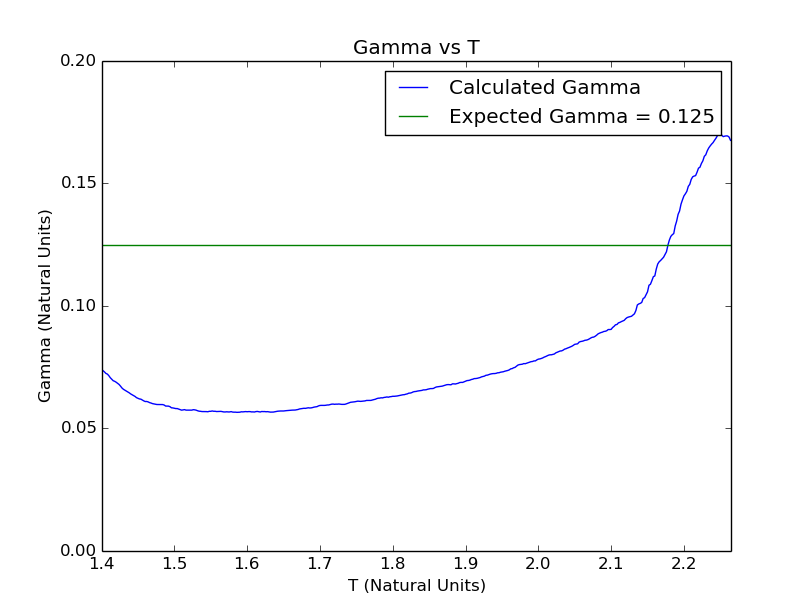
\includegraphics[width= \linewidth]{log_mag_v_log_tmtc.png}
\end{minipage}\hfill
\caption{Plot of log(m) versus log(abs(T-Tc)).}
\label{fig:figure5}
\end{figure}
\n

\section{Conclusion}
Using the Wolff algorithm on a finite, periodic lattice, the temperature dependence of magnetization, susceptibility, internal energy, and heat capacity can be found.  The critical temperature was found to be 2.285 (in natural units) which is the temperature at which susceptibility is minimal.  The critical exponent $\gamma$ was found to be 0.1 which is close to the expected 0.125.

	



\end{document}